\documentclass{article}

\usepackage[latin1]{inputenc}
\usepackage[english]{babel}
\usepackage{algorithm}
\usepackage{algpseudocode}  % pseudocode (aus algorithmixs)
\usepackage{graphicx}
\usepackage{amsmath}


\newcommand{\latvec}{\textsc{LatVec}}

\newsavebox{\savepar}
\newenvironment{boxit}{\begin{lrbox}{\savepar}\begin{minipage}[t]{0.8\textwidth}}
                      {\end{minipage}\end{lrbox}\fbox{\usebox{\savepar}}}

\title{\latvec{} - Manual}

\date{}

\author{Martin Mann - University Freiburg \\\\
{http://www.bioinf.uni-freiburg.de/}}

\begin{document}

\maketitle


\begin{center}
  \textsc{LatPack} Tools Package
  
  Version 1.9.1
\end{center}


\section{Description}

\latvec{} implements a chain growth algorithm to simulate Sequential Folding
of lattice proteins (see \cite{Mann:latpack:HFSP08}). It supports:
 
\begin{enumerate}
  \item various lattices (see Sec.~\ref{sec:lat})
  \item arbitrary energy functions (see Sec.~\ref{sec:energy})
  \item side chain models
  \item PDB (Protein Data Bank) output of the best structure found
  \item check for extensibility of last appended monomer
  \item symmetry exclusion via move string normalization
  \item extension of all structures within a given energy interval above the
  minimal energy reachable so far
\end{enumerate}

\section{Method}
\label{sec:method}

\latvec{} implements a greedy heuristic of a chain-growth approach. The
mo\-no\-mers are placed successively on lattice positions such that the
structure forms a selfavoiding walk. For each length all possible structure extensions
with one monomer are generated and evaluated. The best structures are considered
in the next extension iteration. The process is described in more detail in
Sec.~\ref{sec:ext}

Due to the lattice restrictions and the selfavoidingness constraint, the
procedure may end in non-extensible structures during the iteration and fail. A
fast way to overcome this problem is to check the extensibility of the last
monomer after its placement. Only extensible structures are considered further
and evaluated later. A cheap form of extensibility check is presented in
Sec.~\ref{sec:endCheck}.

A description what kind of energy functions are supported is given in
Sec.~\ref{sec:energy}. Furthermore, the text file format for the different
function types is specified to allow for arbitrary energy functions by the user.

\subsection{Chain Growth Algorithm - Backbone Model}
\label{sec:ext}

\subsubsection*{Given:}

\begin{tabular}{rcl}
	$S=S_1,\ldots,S_n$ &:& monomer sequence from alphabet $A$ to fold \\
	$E(S,P)$ &:& energy function (see Sec.~\ref{sec:energy})\\
	$N$ &:& the neighboring vectors of the lattice model to use \\
	$\Delta E$	&:& energy interval above the minimal energy for this \\
				&& iteration that are going to be extended in the next
\end{tabular}

\subsubsection*{Result:}

\begin{tabular}{rcl}
	$L=L_1,\ldots,L_n$	&:& 3D coordinates of the energetically best sequential \\
						&& placement of $S$ in the lattice
\end{tabular}

\subsubsection*{Method:}

The approximation follows a greedy structure-elongating chain-growth approach:

\vspace{0.5em}
\begin{algorithmic}[1]
	\State $B \gets \{L_1=(0,0,0)\}$ \Comment{best structures of last
	iteration} \Statex \Comment{initialized by placing the first
	monomer to $(0,0,0)$}
	\State $C \gets \emptyset$ \Comment{structures generated in current iteration}
	\For{$i = 2 \ldots n$}
		\ForAll{$L \in B$} \Comment{$L$ has length $(i-1)$}
			\ForAll{$\vec v \in N$}
				\If{$L_{(i-1)} + \vec v \not\in \{L_1,\ldots,L_{(i-1)}\}$} 
				\Comment{selfavoidingness}
					\State $L' \gets (L_1,\ldots,L_{(i-1)},L_{(i-1)} + \vec v)$
					\State $C \gets C \cup \{L'\}$
					\Comment{store normalized extension}
				\EndIf
			\EndFor
		\EndFor
		\State $minE \gets $ minimal energy of all elements in $C$ 
		\State $B \gets \{ c \;|\; c\in C $ and $E(S_{1\ldots i},c) \leq (minE+\Delta
		E)\}$
		\Comment{copy all best}
		\State $C \gets \emptyset$ \Comment{reset structure storage}
	\EndFor
	\State report best placement $L \in B$ with minimal energy $E(S,L)$
\end{algorithmic}

\vspace{1em}
{\bfseries Note:} Due to the greedy storing of the energetically best structures
only, it may occure that none of the structures in $B$ can be extended in a
selfavoiding way (Line~6 gives 'false'). Therefore, $C$, and in the
following~$B$, would get empty and the procedure stops without finding a
selfavoiding walk of the whole sequence~$S$. This problem can usually be solved
either by increasing $\Delta E$ or by adding an extensibility check in line~6.
Both results in additional computations and an increased runtime.


\subsection{Extensibility Check}
\label{sec:endCheck}

A first and cheap variant of extensibility check is to verify that the
position of the last appended monomer has at least one free neighbored. This
ensures that at least one additional monomer can be added.

But, this is \emph{not} enough to \emph{ensure} extensibility. Still it
might be the case that the current placement of the last monomer only allows a
limited extension of the chain, not sufficient to place all remaining monomers.

Nevertheless, this check seems to be sufficient in general and the described
scenario may only occure for long sequence lengths. The minimal length that
makes such a placement possible strongly depends on the lattice model and the
size of the corresponding neighborhood, i.e. number of neighboring vectors. In
the square lattice, the minimal length is~10. The corresponding structure is
given in Fig.~\ref{fig:squareStucked}. The last appended (red) monomer has a
free neighbored position (yellow), but this position has none and will not be
extensible. This situation cannot be determined using the simple check. Here, a
full extensibility check that validates if there is a free path out of the
structure has to be done.

\begin{figure}[H]
\begin{center}
	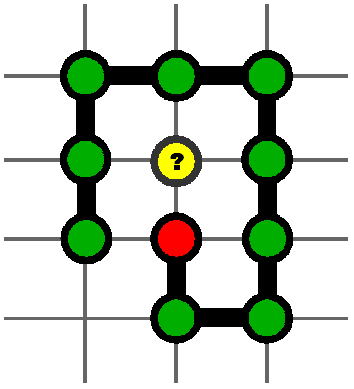
\includegraphics[width=0.3\textwidth]{square-stucked}
	\caption{Non-extensible structure in the 2D-square lattice that is not
	rejected by the simple extension check. Here the last position (red) can be
	extended (yellow position). But afterwards no extension will be possible any
	more.}
	\label{fig:squareStucked}
\end{center}
\end{figure}


\subsubsection*{Given:}

\begin{tabular}{rcl}
	$L=L_1,\ldots,L_n$	&:& 3D coordinates of a lattice protein structure \\
	$N$ &:& the neighboring vectors of the lattice model to use \\
\end{tabular}

\subsubsection*{Result:}

\begin{tabular}{rcl}
	\textsc{true/false} &:& whether or not position $L_n$ has a free neighbored
	position
\end{tabular}

\subsubsection*{Method:}

The approach performs a full check of all neighbored positions if necessary :

\vspace{0.5em}
\begin{algorithmic}[1]
	\ForAll{$\vec v \in N$}
		\State $i \gets 1$
		\State $isFree \gets$ \textsc{TRUE}
		\While{$i < n$ and $isFree$}
			\State $isFree \gets L_i \neq (L_n + \vec v)$ 
			\Comment{check if occupied}
			\State $i \gets i+1$
		\EndWhile
		\If{$isFree = $ \textsc{TRUE}}
			\State\Return{\textsc{TRUE}} \Comment{this neighbored position is free}
		\EndIf
	\EndFor
	\State \Return{\textsc{FALSE}} \Comment{no free neighbored position found}
\end{algorithmic}



%%#############################################################################
%%#############################################################################
\subsection{Symmetry exclusion via normalization}
\label{sec:moveNormalization}
%%#############################################################################
%%#############################################################################


The normalization is done indirectly via a conversion of the 3D coordinates into
absolute move string representation. Here, a string is produced that represents
the neighboring vectors between successive monomer coordinates. The resulting
move string is normalized based on the neighboring and automorphism information
of the given lattice. This information is used to create move exchange tables for
each automorphism which is utilized to determine the lexicographically smallest
symmetrical move string. The reconversion of this normalized move string into 3D
coordinates results in the unique symmetrical (normalized) structure.



%%#############################################################################
%%#############################################################################
\section{Available Lattices}
\label{sec:lat}
%%#############################################################################
%%#############################################################################

Several lattice models can be used to fold a structure. 

\vspace{0.5em}
The currently supported lattice models and the corresponding neighboring
vectors are:

\vspace{0.5em}
\begin{tabular}{c|l|l|c}
	ID & Name & Neighborhood vectors & \#\\
	\hline
	SQR & Square & $\{\pm(1,0,0),\pm(0,1,0)\}$ & 4\\
	CUB & Cubic & $\{\pm(1,0,0),\pm(0,1,0),\pm(0,0,1)\}$ & 6\\
	FCC & Face Centered Cubic & 
	$\left\{\pm(1,1,0),\pm(1,0,1),\pm(0,1,1), \atop
	\pm(1,-1,0),\pm(1,0,-1),\pm(0,1,-1)\right\}$ & 12 
\end{tabular}



\section{Energy Functions}
\label{sec:energy}

\latvec{} supports arbitrary energy functions that are based either on contacts
or on distance intervals. The specification of an energy function has to be
given in text format and defines the allowed sequence alphabet as well.

In general, the energy of a sequence~$S$ of length~$n$ with structure
coordinates~$P$ is determined by
\begin{equation}
	E(S,P) = \sum_{1\leq i+1<j\leq n} e(S_i, S_j, P_i, P_j).
\end{equation}
Here, $e(S_i, S_j, P_i, P_j)$ is a placeholder for the specific evaluation
function that is given for the different types in the following.

\subsection{Contact Based Energy Function}
\label{sec:energy:contact}

A contact based energy function for an alphabet $A$ is defined by an energy
table $E^c : |A|\times|A| \rightarrow \mathcal{R}$ such that 

\begin{equation}
	e_c(S_i, S_j, P_i, P_j) = 
	\left\{
	\begin{array}{ll}
    	E^c[S_i,S_j] & \mbox{ if $P_i$ and $P_j$ are neighbored} \\
    	0 & \mbox{ else }
    \end{array} \right.
\end{equation}

For example, a function like this was used by Lau and Dill to define the widely
used HP-model~\cite{Lau_Dill:89a}.

\subsubsection*{\underline{ Text File Encoding }}

The \latvec{} text file enconding of a contact based energy function consists of
two parts: the alphabet elements and the energy table. A consecutive string of
the alphabet elements in the first line determines the allowed protein sequence
characters (the alphabet) and the dimensions of the energy table that is read
from the remaining file.

An example energy file for the HPNX-model is:

\begin{center}
\begin{boxit}
\small
\begin{verbatim}
HPNX
-4.0  0.0  0.0  0.0
 0.0 +1.0 -1.0  0.0
 0.0 -1.0 +1.0  0.0
 0.0  0.0  0.0  0.0
\end{verbatim}
\end{boxit}
\end{center}


\subsection{Distance Interval Based Energy Function}
\label{sec:energy:distance}

A distance insterval based energy function for an alphabet $A$ is defined by a
consecutive set of~$k$ distance intervals with the upper bounds~$d^{up}_{1\ldots
k}$ and an energy table $E^i_{1\ldots k} : |A|\times|A| \rightarrow \mathcal{R}$
for each of them. Given the distance to interval index function $idx$ we define
the evaluation function

\begin{eqnarray}
	e_i(S_i, S_j, P_i, P_j) & = & E^i_{idx(P_i,P_j)}[S_i,S_j] \\
	idx(P_i,P_j) & = & \arg\min_{k}\;(|P_i-P_j| \leq d^{up}_k)
\end{eqnarray}


\subsubsection*{\underline{ Text File Encoding }}

The \latvec{} text file enconding of a distance interval based energy function
consists of three parts: the alphabet elements, the upper bounds of the intervals
and the energy tables for the interval. A consecutive string of the alphabet
elements in the first line determines the allowed protein sequence characters
(the alphabet) and the dimensions of the energy tables. The second line
contains a whitespace separated list of the upper interval bounds. Their number
sets the number of energy tables read from the remaining file. The interval
bounds are expected to be given in {\AA}ngstroems. For a correct scaling of
the bounds it is necessary to give the average distance of two consecutive
$C_\alpha$-atoms in the underlying model to \latvec{} (see input parameters in
Sec.~\ref{sec:parameter}).

An example energy file that encodes the HPNX-model using a distance interval
based energy function is:

\begin{center}
\begin{boxit}
\small
\begin{verbatim}
HPNX
3.7 3.9 999999

 0.0  0.0  0.0  0.0
 0.0  0.0  0.0  0.0
 0.0  0.0  0.0  0.0
 0.0  0.0  0.0  0.0

-4.0  0.0  0.0  0.0
 0.0 +1.0 -1.0  0.0
 0.0 -1.0 +1.0  0.0
 0.0  0.0  0.0  0.0

 0.0  0.0  0.0  0.0
 0.0  0.0  0.0  0.0
 0.0  0.0  0.0  0.0
 0.0  0.0  0.0  0.0
\end{verbatim}
\end{boxit}
\end{center}

The number $999999$ is used as a placeholder for $+\infty$, i.e. the upper bound
of the last distance interval. It is important to know that the average
$C_\alpha$-distance in the underlying model was 3.8~\AA. Therefore, the resulting
interval energy function corresponds to the contact based energy function of the
previous section; only distances close to the average $C_\alpha$-distance are
taken into account.


\section{Program Parameters}
\label{sec:parameter}

\subsubsection*{\underline{ Input }}

\begin{description}
	\item[-seq] The sequence to fold co-translationally. It has to be conform
	to the alphabet given by the energy file (see {\bfseries -energyFile}).
	\item[-energyFile] A file that encodes the used alphabet and the
	specific energy function (see Sec.~\ref{sec:energy} for format details).
	\item[-energyForDist] If present, the input of {\bfseries -energyFile} will be
	interpreted as distance interval energy function. Otherwise a contact based
	energy functino is expected.
	\item[-energyCalphaDist] Specifies the average distance of two
	consecutive $C_\alpha$-atoms in the underlying model. This value is needed to
	scale the intervals of a distance interval based energy function onto the
	$C_\alpha$-distances of the lattice model in use.
\end{description}


\subsubsection*{\underline{ Lattice Settings }}

\begin{description}
	\item[-lat] The lattice model to use for the sequential folding. The
	available list of lattice identifiers is given in Sec.~\ref{sec:lat}.
\end{description}


\subsubsection*{\underline{ Side Chain Settings }}

\begin{description}
	\item[-sideChain] If present, a representation of two monomers per amino acid
	is done. One for the backbone atoms and one representing the side chain. 
\end{description}


\subsubsection*{\underline{ Chain Growth Parameters } (see Method
Sec.~\ref{sec:method})}

\begin{description}
	\item[-deltaE] Energy interval above the minimal energy found. Only structures
	with an energy within this interval are extended in the next iteration.
	\item[-noExtCheck] If present, no check for extensibility of the last monomer
	is done. Otherwise, the last appended backbone monomer is checked to have at
	least one free neighbored position.
	\item[-extMax] The maximal number of structures that are going to be extended
	in the next iteration. This parameter only influences the memory consumption
	of \latvec{} by restricting the size of the candidate set $C$ of the algorithm
	(see Sec.~\ref{sec:ext}). If $C$ exeeds the given size, the chain growth is
	stopped. Note, both sets, $B$ and $C$, can maximally contain the given number
	of candidate structures.
	\end{description}


\subsubsection*{\underline{ Output }}

\begin{description}
	\item[-print] The number of final structures to print maximally in the end. The
	structures are given in absolute moves to reduce space consumption. The move
	encoding is:\\\\
	\begin{tabular}{c|c}
    	move & neighbor vector \\
    	\hline
    	L & $(+1,0,0)$ \\
    	R & $(-1,0,0)$ \\
    	F & $(0,+1,0)$ \\
    	B & $(0,-1,0)$ \\
    	U & $(0,0,+1)$ \\
    	D & $(0,0,-1)$ 
    \end{tabular}
	\item[-printBest] If present, only the structures with minimal energy are
	printed.
	\item[-best2PDB] If present, it defines the file to that the best structure is
	written in PDB-format. Here, all monomers are considered to be a Histidine
	amino acid.
\end{description}


\subsubsection*{\underline{ Miscellaneous }}

\begin{description}
	\item[-v] Give verbose output during computation.
	\item[-s] Give only minimal output during computation.
	\item[-help] Prints the available program parameters.
\end{description}


\section{Contact}

\begin{tabular}{lcr}
	Martin Mann  && \bfseries http://www.bioinf.uni-freiburg.de/\\
	Bioinformatics Group\\
	University Freiburg, Germany \\
\end{tabular}





\begin{thebibliography}{99}
\bibitem{Lau_Dill:89a}{
	  Kit Fun Lau and Ken A. Dill:
	  {\bfseries A Lattice Statistical Mechanics Model of the Conformational 
	  and Sequence Spaces of Proteins}, 
	  \emph{Macromolecules} 1989,
	  {\bfseries 22}(10):3986--3997
	 }
\bibitem{Mann:latpack:HFSP08} {
	Mann, M., Maticzka, D., Saunders, R., and Backofen, R.:
	{\bfseries Classifying protein-like sequences in arbitrary lattice protein models using {LatPack}},
	\emph{HFSP Journal} 2008, {\bfseries 2}(6), 396.
	Special issue on protein folding: experimental and theoretical approaches
	}
% \bibitem{Miao.et.al:JMB:H-collapse:04}{
% 	  J.~Miao, J.~Klein-Seetharaman and H.~Meirovitch:
% 	  {\bfseries The Optimal Fraction of Hydrophobic Residues Required to Ensure
% 	  Protein Collapse}, \emph{Journal of Molecular Biology}
% 	  2003,
% 	  {\bfseries 344}:797-811
% 	 }
% \bibitem{Godzik.et.al:JCC:globLat:93}{
% 	  A.~Godzik, A.~Kolinski and J.~Skolnick:
% 	  {\bfseries Lattice Representations of Globular Proteins: How Good Are They?},
% 	  \emph{Journal of Computational Chemistry} 1993,
% 	  {\bfseries 14(10)}:1194-1202
% 	 }
\end{thebibliography}
 

\end{document}